\documentclass[11pt,a4paper]{article}

\usepackage[utf8]{inputenc}
\usepackage[T1]{fontenc}
\usepackage[margin=1in]{geometry}
\usepackage{amsmath,amssymb}
\usepackage{booktabs}
\usepackage{graphicx}
\usepackage{hyperref}
\usepackage{xcolor}
\usepackage{caption}
\usepackage{array}

\hypersetup{
    colorlinks=true,
    linkcolor=blue!60!black,
    citecolor=blue!60!black,
    urlcolor=blue!60!black
}

\title{\textbf{From Connectome Wiring to Counted Memory and Recurrent Depth:\\Pre-Registered Tests of \emph{Drosophila} Mushroom-Body Principles\\in Small Language Models}}
\author{Nate \\ \small Independent Researcher}
\date{17 November 2026}

\begin{document}
\maketitle

\begin{abstract}
Biological neural circuits inspire machine learning both as literal connectivity graphs and as algorithmic motifs---sparse random expansion, homeostatic competition, fast associative memory, and adaptive recurrent computation. Across \textbf{16 pre-registered stages} (101 production training and evaluation runs, \textbf{25 registered predictions P1--P25}, and a \textbf{218-mutant automated test audit}), we systematically test where \emph{Drosophila} mushroom-body principles help---and where they fail---in small language models (5M--29M parameters trained on 200M tokens of FineWeb-Edu).

First, in \textbf{Stage 1} and \textbf{Stage 2T}, replacing a 6-layer transformer's feed-forward networks with a shared recurrent reservoir wired like the adult \emph{Drosophila} mushroom body (FlyWire v783: 6,293 neurons, 570,682 synapses) performs \textbf{reliably worse} than degree-preserving random shuffles ($\text{real} - \text{shuf} = +0.0126, +0.0147, +0.0160$ nats/token, verdict \texttt{X\_WORSE}) and dense or Erd\H{o}s--R\'enyi controls ($\text{dense} < \text{er} < \text{real\_randio} \approx \text{shuf} < \text{real}$). While the real connectome has half the effective rank of its shuffles ($0.48\times$), its full-brain activity participation ratio equals the shuffles ($\text{real} \div \text{shuf} = 1.00$, refuting P1); instead, its three-layer anatomical routing ($\text{ALPN} \to \text{KC} \to \text{MBON}$) leaves only \textbf{19.5\%} of readout neurons one hop from an input (versus \textbf{95.5\%} in degree-preserving shuffles), delaying readout dimensionality by one recurrent step.

Second, in \textbf{Stages 2.0--2B and 2E--2K2}, we replace literal connectome wiring with a counted host-RAM $n$-gram memory (\textbf{COUNT}, orders 2--5 over 881M tokens, 5.15 GiB host RAM, zero GPU parameters) and test a mushroom-body similarity backoff (\textbf{Kenyon hash}: fixed PPMI token codes, sparse random expansion $K=31$, homeostatic $k$-winners-take-all into $4.19\times 10^6$ buckets). Online \textbf{leave-one-out} count subtraction during training is essential, preventing a \textbf{+0.84 nat} validation collapse from target leakage. On equally tuned separate learning rates (Muon $8\times 10^{-3}$ on block matrices, AdamW $64\times 10^{-3}$ on embeddings and head), plain COUNT lowers 13.8M-parameter (\texttt{Size M}) validation loss by \textbf{$-0.1224$ nats} ($3.3853 \to 3.2629$, \texttt{X\_BETTER}, P12--P13), matching a \textbf{29.4M-parameter (\texttt{Size L})} baseline at $+3.4\%$ step time and zero additional VRAM. However, while the Kenyon similarity backoff improves an offline $n$-gram model on unseen and rare histories ($+0.0151$ and $+0.0130$ nats, P5 supported), that gain \textbf{vanishes inside the neural network} ($+0.0046$ nats vs plain COUNT, \texttt{NO\_MEANINGFUL\_DIFFERENCE}, P4 refuted). Likewise, learned per-order/per-bin gates and scalar controls (\textbf{Stages 2E, 2K, 2K2}) fail to beat plain COUNT once embeddings and the unembedding head train at $64\times 10^{-3}$ (P19--P20 refuted).

Third, in \textbf{Stages 2C, 2C-2, and 2C-3}, we test complementary learning systems (CLS) using gradient-free one-shot count writes (\texttt{Overlay}) followed by KL-anchored replay consolidation into slow weights. One-shot writes learn 4 sequential lists of 384 cue--answer pairs (1,536 pairs) with \textbf{0.760 recall} and \textbf{zero catastrophic forgetting} ($\text{backward transfer} = 0.000$ vs $-0.330$ and $-0.651$ for gradient fine-tuning, P7 supported). We show that standard sequential replay consolidation collapses ($0.061$ recall) due to \textbf{teacher drift} (Stage 2C-2, $+0.704$ recovery with an untouched teacher) and \textbf{overlay-channel drift} (Stage 2C-3, H1a supported: consolidating with the overlay off de-calibrates the backbone's memory-reading pathway, dropping recall on an unseen 5th list from $0.797$ to $0.177$). Adding a \textbf{memory-on KL consistency loss} restores both memory-off ($0.731$) and memory-on ($0.750$) consolidated recall while preserving unseen-list reading ($0.763$). Furthermore, gating test-time overlay writes by stored $n$-gram history counts (\texttt{GatedOverlay}) preserves \textbf{100\% of quiz recall ($0.7602$) while cutting English validation loss interference by 81.0\%} at $C(h_3)\le 0$, and cuts interference by \textbf{95.4\% ($+0.038$ nats)} at $C(h_2)\le 9$.

Fourth, in \textbf{Stages 2D, 2H, 2I, and 2L--2N}, we study recurrent depth (\texttt{LoopGPT}: 2 prelude blocks, a shared 2-block core looped $r \in \{1,\dots,6\}$ times, 2 coda blocks). While exact token-level optimal halting scales affinely with log-effort (P9 supported, $R^2 = 0.957\text{--}0.993$) and beats fixed depth by $0.0626$ nats, \textbf{no deployable causal halting rule} (state-change, entropy, margin, or ridge-regression state probes) beats fixed depth by $0.01$ nats (P18 refuted; linear probes explain $<1\%$ of next-pass benefit variance, and entropy exiting is \texttt{X\_WORSE} by $-0.0305$ nats). Training with a \textbf{learned per-pass residual gain (\texttt{loop\_gain}) and all-depth loss} (Stage 2H, P17 supported) lowers validation loss by \textbf{$-0.0384$ nats} ($3.3720 \to 3.3336$) and learns to damp passes 5--6 to zero automatically, so fixed depth 3 captures \textbf{99.2\%} of the 6-pass gain. Finally, through a pre-registered $2\times 2$ factorial (\textbf{Stages 2M--2N}, P22--P25), we prove that training the untied \texttt{head.weight} at $64\times 10^{-3}$ with zero weight decay causes an \textbf{8$\times$ L2 norm explosion ($>5,200$ vs $\sim 730$)} that locks the shared readout to pass 1 and kills recurrent depth. Restraining \texttt{head.weight} to $8\times 10^{-3}$ (\texttt{SHARED} and \texttt{HEADLOW}) revives the loop ($+0.0376$ and $+0.0309$ nats loop benefit) and achieves \textbf{3.2012 nats} ($3.2015$ at depth 3)---a \textbf{$-0.2029$ nat} total reduction below the \texttt{B0-M} baseline ($3.4041$) at identical GPU parameter count.
\end{abstract}

\section{Introduction and Pre-Registration Protocol}

Every experimental stage in this work (\texttt{Stage 1}, \texttt{Stage 2.0}, and \texttt{Stages 2A} through \texttt{2N}) was pre-registered in a version-controlled \texttt{PREREG\_*.md} document prior to launching production runs. Each run's output JSON records the SHA-256 digest of its config and pre-registration file along with \texttt{git\_dirty: false}. Across all stages, the Smallest Effect Size of Interest (SESOI) was fixed at $0.01$ nats/token (twice the $0.0027$ seed standard deviation of \texttt{B0-M}, where the $0.01$ floor binds). Paired seed comparisons $d_s = L_X(s) - L_Y(s)$ were evaluated automatically by \texttt{clm.analyze.verdict}:
\begin{itemize}
    \item \texttt{X\_BETTER}: $\text{mean}(d) \le -0.01$ and $d_s < 0$ for every seed $s$.
    \item \texttt{X\_WORSE}: $\text{mean}(d) \ge +0.01$ and $d_s > 0$ for every seed $s$.
    \item \texttt{NO\_MEANINGFUL\_DIFFERENCE}: $|\text{mean}(d)| < 0.01$ and $|d_s| < 0.02$ for every seed $s$.
    \item \texttt{INCONCLUSIVE}: all other finite outcomes.
\end{itemize}
To ensure implementation integrity, \texttt{scripts/mutation\_audit.py} plants \textbf{218 single-line bugs (M1--M222)} across \texttt{src/clm/} and verifies that the unit test suite kills $218/218$ mutants by \texttt{AssertionError}.

\section{Part I: Literal Connectome Wiring vs Controls (Stages 1 \& 2T)}

In Stage 1, we replaced the feed-forward networks of a 6-layer pre-norm GPT ($d_{\text{model}}=256$, 4 heads, context 256, BPE vocab 8,192, tied embeddings, 5.11M parameters) with a single \texttt{SharedBrain} reservoir stepped once per layer ($\text{leak}=0.5$, GELU, RMS-normalised across all neurons, state persisting across layers $0\dots 5$ within a token). Five arms were trained for $200\text{M}$ tokens on FineWeb-Edu shard 000 across seeds $0, 1, 2$: \texttt{real} (FlyWire v783 mushroom body: 6,293 neurons, 570,682 synapses), \texttt{shuf} (degree-preserving Maslov--Sneppen shuffle), \texttt{er} (Erd\H{o}s--R\'enyi), \texttt{real\_randio} (\texttt{real} graph with random input/readout neurons), and \texttt{dense} (760-neuron fully connected reservoir, 577,600 synapses).

\begin{figure}[htbp]
    \centering
    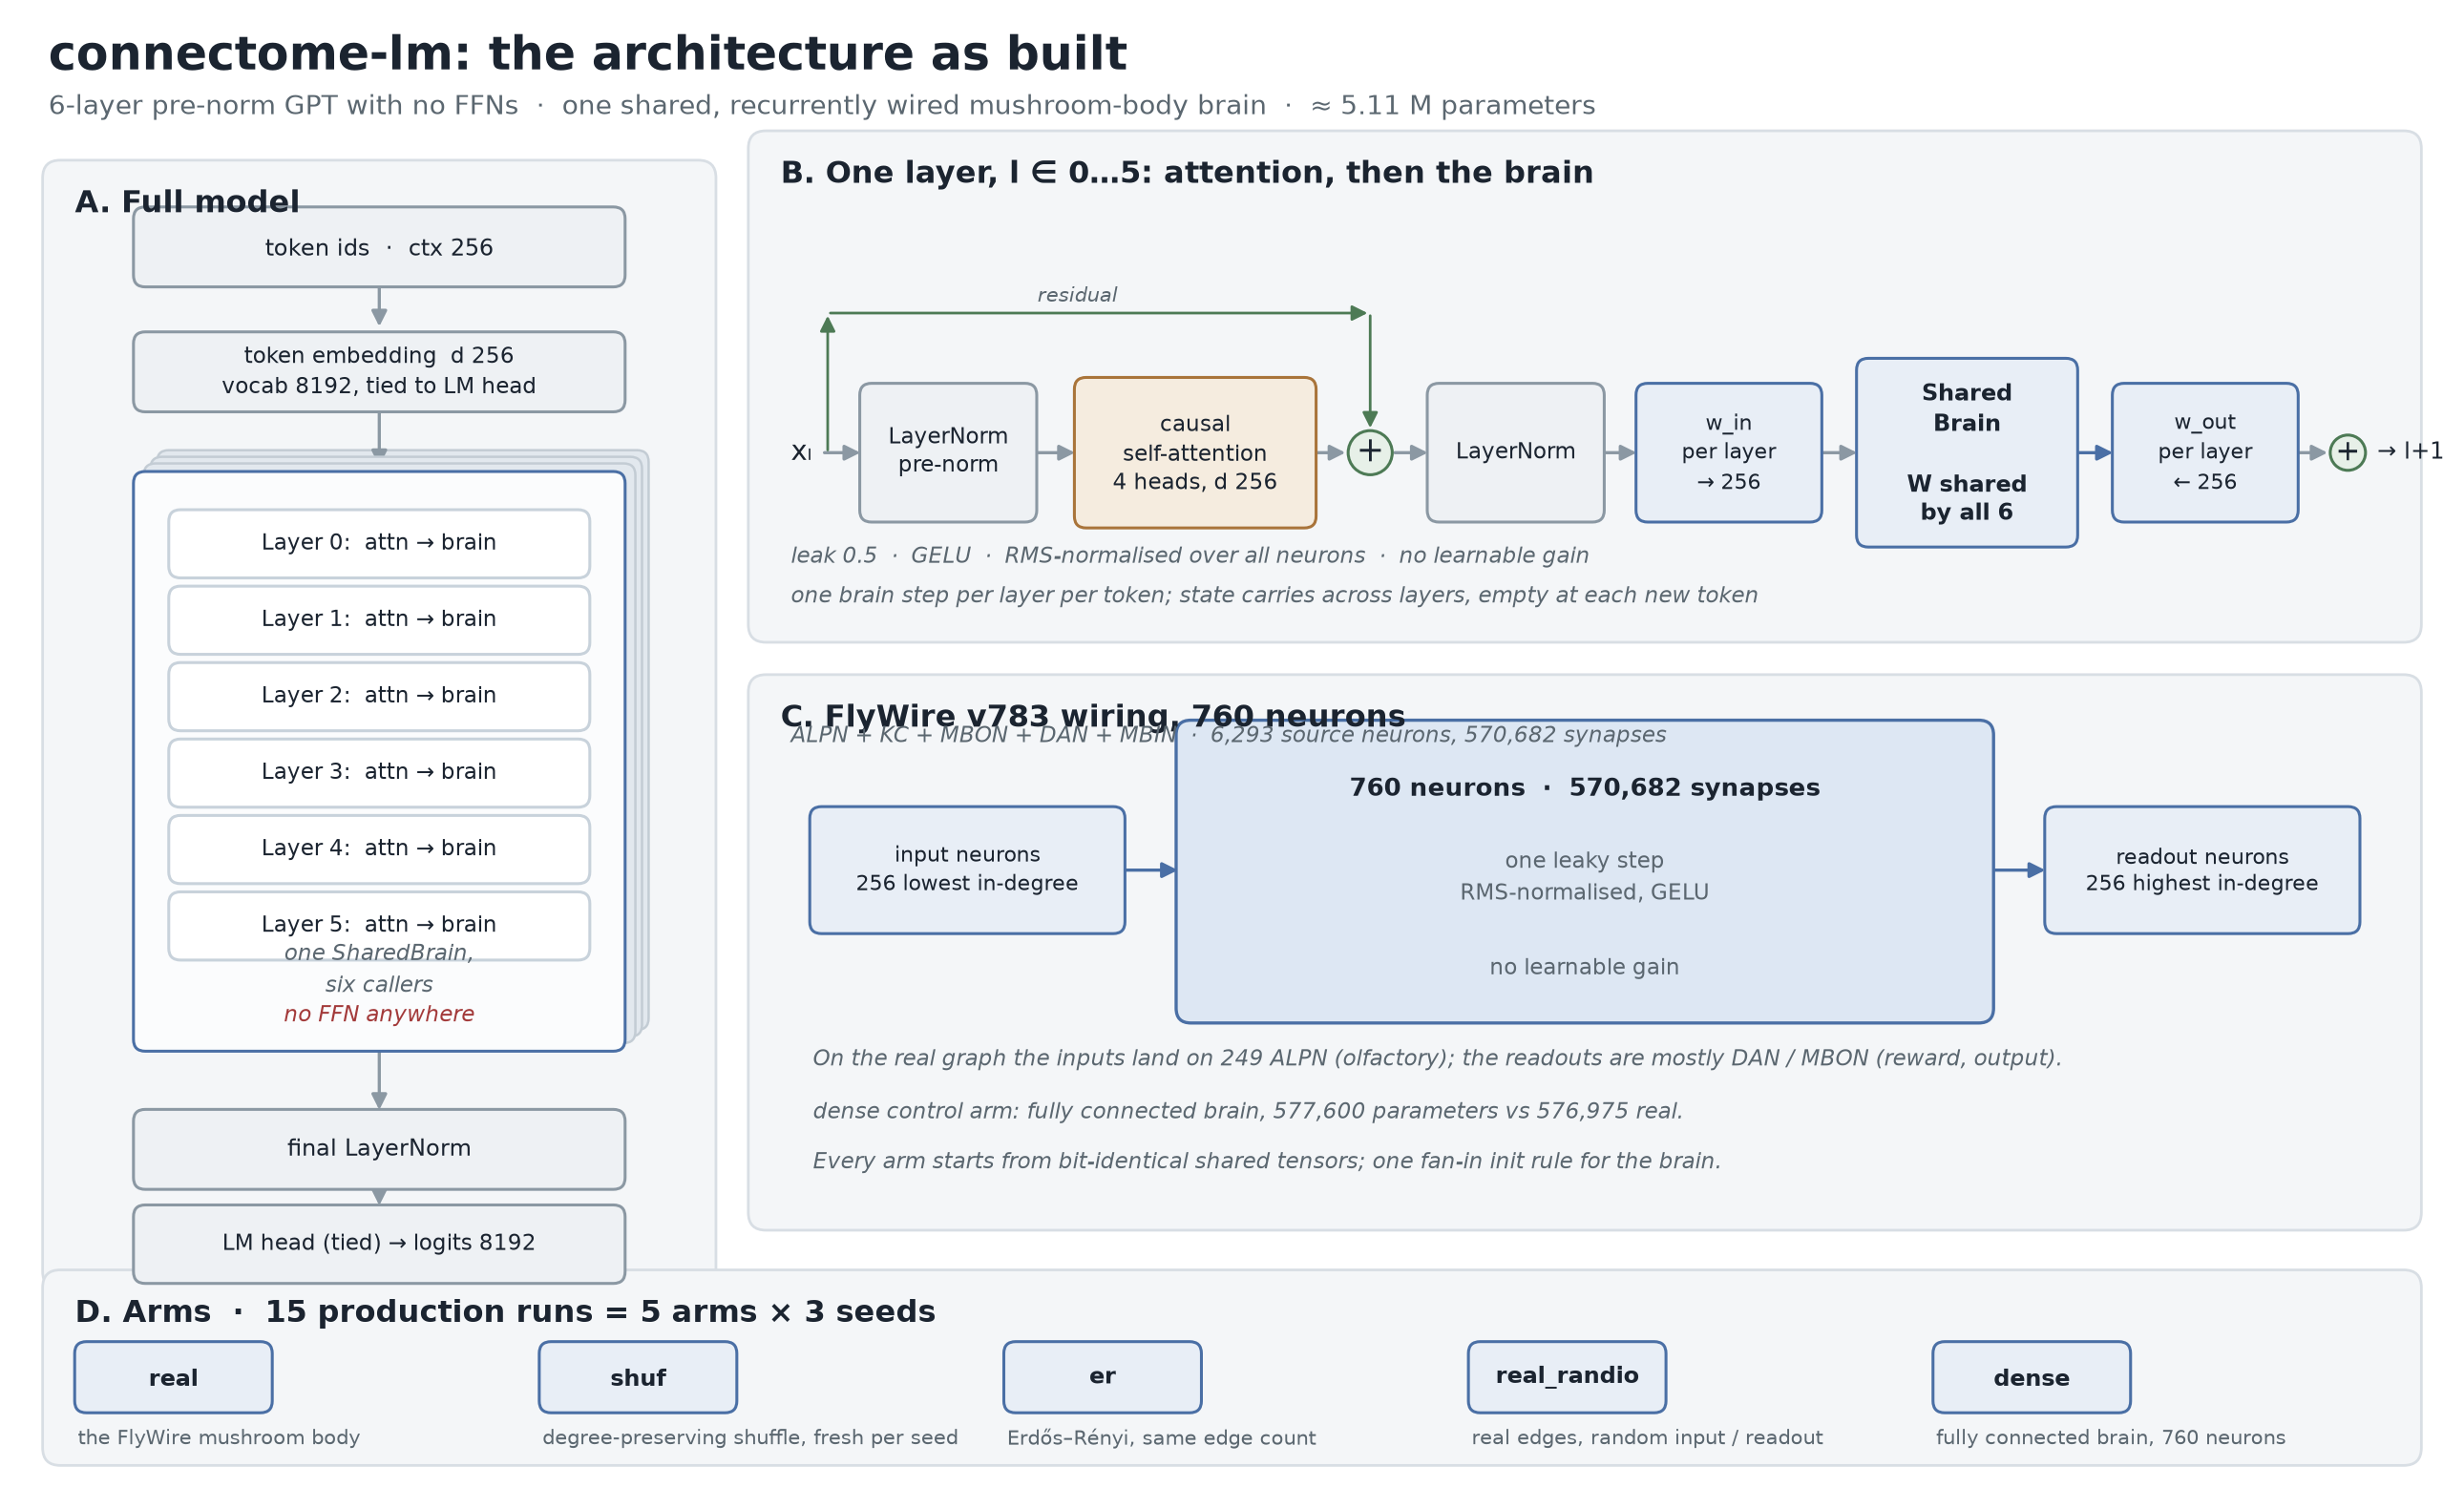
\includegraphics[width=0.98\textwidth]{../docs/architecture_as_built.png}
    \caption{Stage 1 \texttt{connectome-lm} architecture as built (6-layer pre-norm GPT with one recurrent \texttt{SharedBrain} wired from FlyWire v783 mushroom-body connectivity).}
    \label{fig:arch}
\end{figure}

\begin{figure}[htbp]
    \centering
    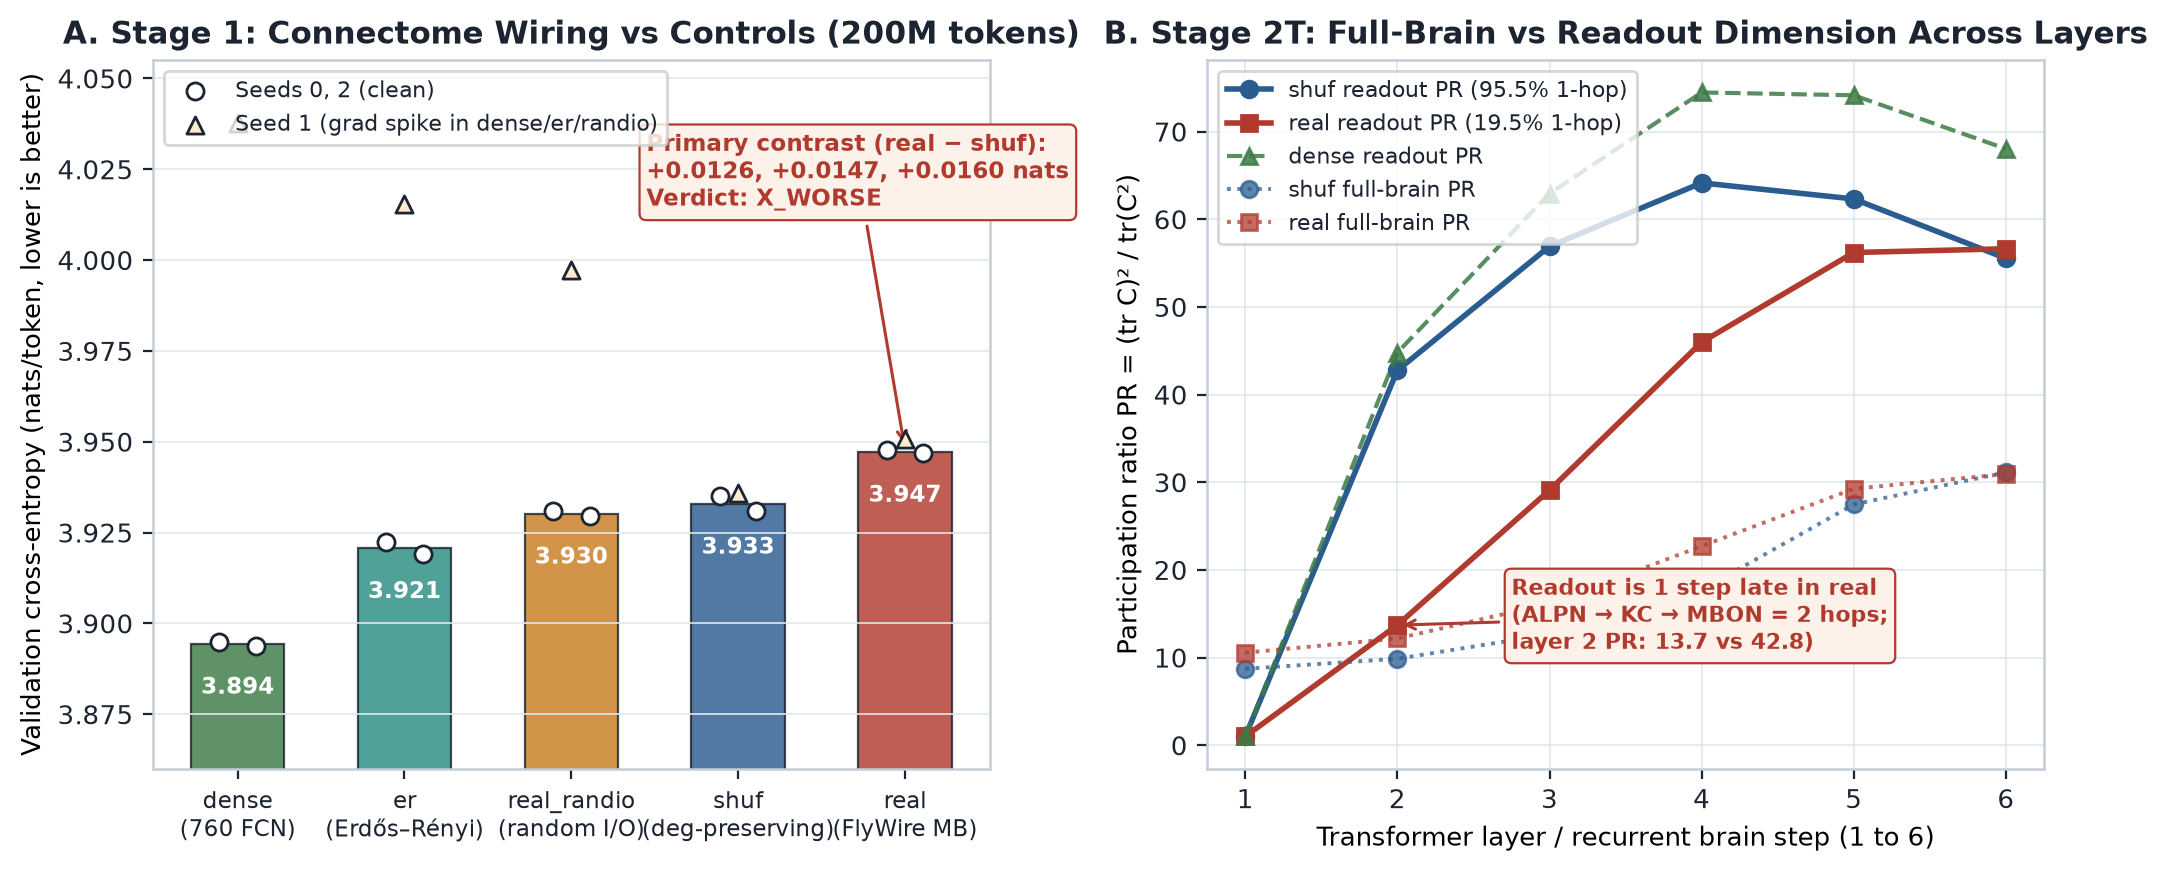
\includegraphics[width=0.98\textwidth]{../docs/figures/fig1_stage1_connectome.png}
    \caption{(A) Stage 1 validation cross-entropy across the five connectome arms. (B) Stage 2T participation ratio $\text{PR} = (\text{tr}\,C)^2/\text{tr}(C^2)$ across layers 1--6 for full-brain versus 256 readout neurons.}
    \label{fig:stage1}
\end{figure}

As shown in Figure~\ref{fig:stage1}, the primary contrast \texttt{real} minus \texttt{shuf} yielded $+0.0126, +0.0147, +0.0160$ nats/token (verdict \texttt{X\_WORSE}). On spike-free seeds 0 and 2, validation loss followed the plasticity-density ordering of Litwin-Kumar et al.\ (2017): $\text{dense} (3.894) < \text{er} (3.921) < \text{real\_randio} (3.930) \approx \text{shuf} (3.933) < \text{real} (3.947)$. Stage 2T refuted the hypothesis (P1) that \texttt{real}'s $0.48\times$ connectivity effective rank halves its activity participation ratio (Layer-6 full-brain $\text{PR}$ ratio $\text{real} \div \text{shuf} = 1.00$), and uncovered an anatomical \textbf{one-step readout delay}: because the biological circuit routes $\text{ALPN} \to \text{KC} \to \text{MBON}$ over two hops, only $19.5\%$ of readout neurons in \texttt{real} lie one hop from an input (vs $95.5\%$ in \texttt{shuf}), depressing readout $\text{PR}$ at Layer 2 from $42.8$ (\texttt{shuf}) to $13.7$ (\texttt{real}).

\section{Part II: Counted Host-RAM Memory, Leave-One-Out, and Fly-Hash Backoff (Stages 2.0--2B, 2E--2K2)}

Moving from literal connectome simulation to hardware-aligned algorithms, Stage 2.0 established a modern transformer baseline (\texttt{B0}: RMSNorm, RoPE, QK-norm, $\text{ReLU}^2$, untied \texttt{head.weight}, value embeddings, logit softcap 30, Muon $8\times 10^{-3}$) across sizes S ($6.82\text{M}$, $3.5198$ nats), M ($13.76\text{M}$, $3.4041$ nats), and L ($29.36\text{M}$, $3.2610$ nats), fitting $L(N) = 8.031\,N^{-0.05235}$.

In Stage 2A, we built host-RAM \textbf{COUNT} tables (orders 2--5, $c_{\min}=(1,1,2,2)$, top-16 continuations, $5.15\text{ GiB}$ over $881\text{M}$ training-split tokens) projected through \texttt{head.weight}. Because the $200\text{M}$-token training stream is a subset of the $881\text{M}$-token count corpus, \textbf{online leave-one-out (LOO)} subtraction during training was mandatory: omitting LOO caused massive target leakage (training loss $2.3967$, validation loss $4.1612$, $+0.8391$ nats worse than with LOO). Decoupling AdamW ($64\times 10^{-3}$) from Muon ($8\times 10^{-3}$) in Stages 2F and 2G lowered \texttt{COUNT-M} loss by $-0.0614$ nats (P12) and widened the paired \texttt{COUNT-M} vs \texttt{B0-M} lead to \textbf{$-0.1224$ nats} ($3.2629$ vs $3.3853$, \texttt{X\_BETTER}, P13), matching \texttt{B0-L} ($29.4\text{M}$) at $+3.4\%$ step time and zero GPU VRAM.

\begin{figure}[htbp]
    \centering
    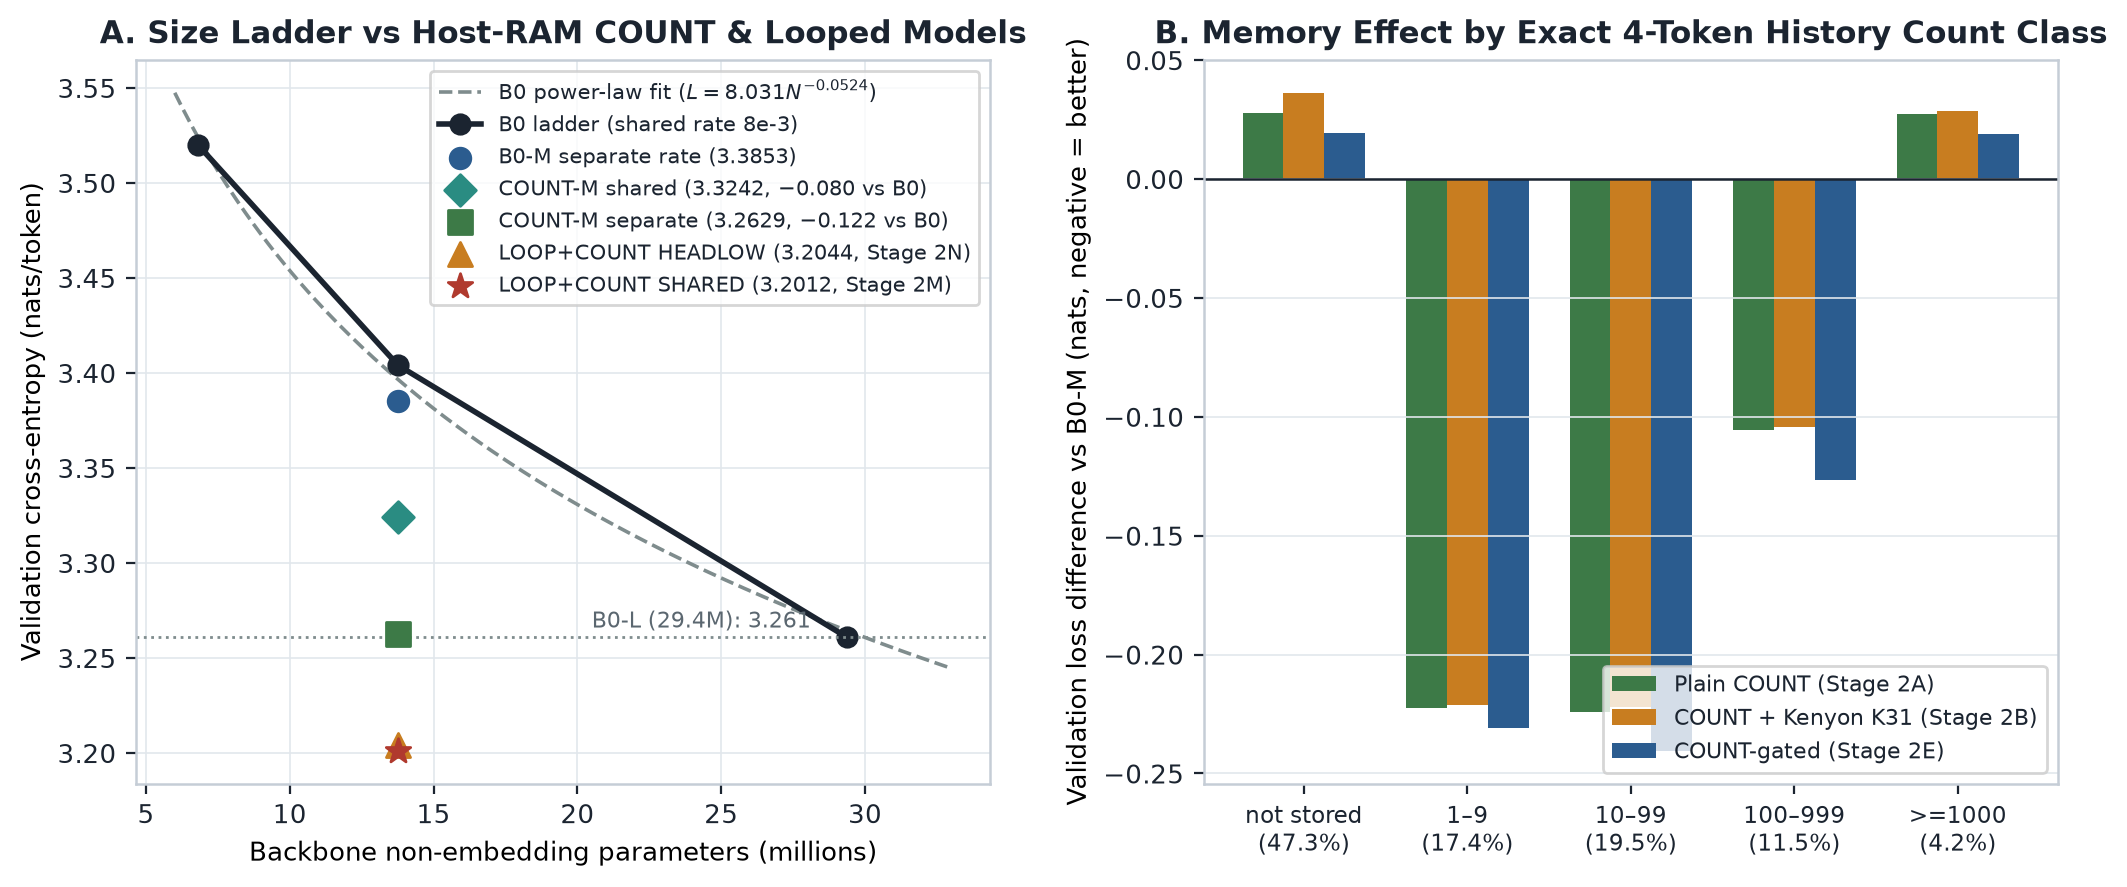
\includegraphics[width=0.98\textwidth]{../docs/figures/fig2_memory_ladder_and_classes.png}
    \caption{(A) B0 size ladder vs host-RAM COUNT and looped models at Size M ($13.8\text{M}$ backbone parameters). (B) Validation cross-entropy difference vs B0-M across exact 4-token history count classes.}
    \label{fig:memory}
\end{figure}

Testing a mushroom-body \textbf{Kenyon similarity backoff} ($K=31$ sparse projection from 64-dim PPMI token codes into $2\times 2,048$ homeostatically balanced cells) improved an offline $n$-gram model on unseen and rare histories by $-0.0151$ and $-0.0130$ nats (Stage 2B-0, supporting $K$-saturation P5 but missing the $0.02$ Gate 2 bar) and made \textbf{no meaningful difference inside the neural network} (Stage 2B: $+0.0046$ nats vs plain COUNT, P4 refuted). Likewise, learned per-order/per-bin gates and scalar controls (Stages 2E, 2K, 2K2) lost to or tied with plain COUNT once \texttt{head.weight} trained at $64\times 10^{-3}$ (P19--P20 refuted).

\section{Part III: Complementary Learning Systems --- One-Shot Writes, Consolidation, and Context Gating (Stages 2C, 2C-2, 2C-3)}

In Stage 2C, one-shot count writes (\texttt{Overlay}, $w=4.0$) learned 4 sequential lists of 384 cue--answer pairs with \textbf{0.760 recall} and \textbf{0.000 backward forgetting} (vs $-0.330$ and $-0.651$ for gradient fine-tuning, P7 supported), while Kenyon 1-token hash writes enabled $3.0\%$ semantic twin transfer without loss of discrimination (P8 supported).

\begin{figure}[htbp]
    \centering
    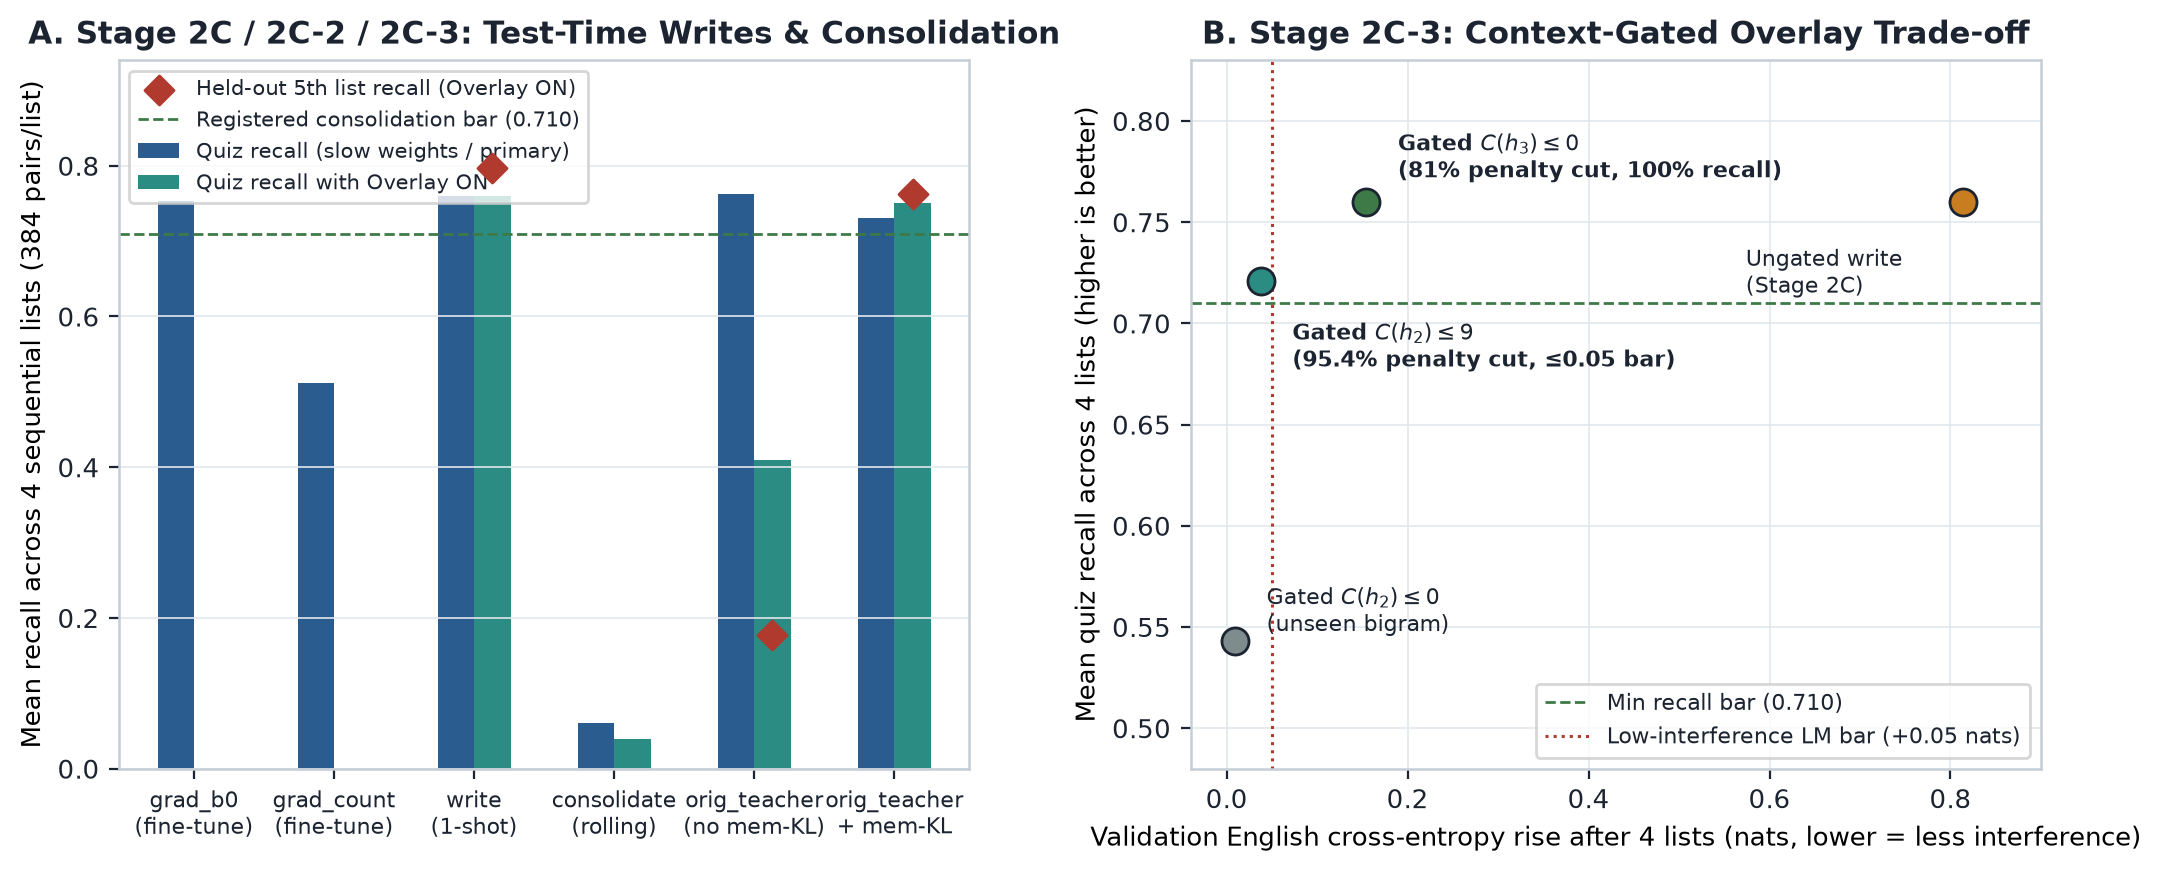
\includegraphics[width=0.98\textwidth]{../docs/figures/fig3_cls_consolidation.png}
    \caption{(A) Sequential list recall and held-out 5th-list recall across gradient fine-tuning, one-shot writes, rolling-teacher consolidation, untouched-teacher consolidation, and memory-on KL consistency repair. (B) Context-gated overlay trade-off between quiz recall and English validation loss rise.}
    \label{fig:cls}
\end{figure}

Stages 2C-2 and 2C-3 diagnosed why sequential KL-replay consolidation initially failed ($0.061$ recall): (1) \textbf{rolling-teacher drift} (Stage 2C-2: keeping the untouched checkpoint as teacher lifted memory-off recall by $+0.704$ to $0.765$), and (2) \textbf{overlay-channel de-calibration} (Stage 2C-3, H1a supported: consolidating with \texttt{overlay=None} broke the student's ability to read the overlay, dropping recall on an unconsolidated 5th list from $0.797$ to $0.177$). Adding a \textbf{memory-on KL consistency loss} (\texttt{memory\_kl\_weight=1.0}) restored memory-off ($0.731$), memory-on ($0.750$), and unseen 5th-list ($0.763$) recall simultaneously. In Part 4b, gating 1-token overlay writes by stored corpus $n$-gram counts (\texttt{GatedOverlay}) preserved \textbf{100\% of quiz recall ($0.7602$) while cutting English validation loss rise by 81.0\%} at $C(h_3)\le 0$, and cut interference by \textbf{95.4\% ($+0.038$ nats)} at $C(h_2)\le 9$ (Figure~\ref{fig:cls}B).

\section{Part IV: Recurrent Depth, Halting Frontiers, and the \texttt{head.weight} Norm Collapse (Stages 2D, 2H--2I, 2L--2N)}

In Stage 2D and Stage 2H, we studied \texttt{LoopGPT} (2 prelude blocks, a shared 2-block loop run $r \in \{1,\dots,6\}$ times, 2 coda blocks). Adding a learned per-pass residual gain (\texttt{loop\_gain}, $6\times 384$) and training on the mean loss over all six depths (Stage 2H \texttt{both}) lowered best-depth validation loss by \textbf{$-0.0384$ nats} ($3.3720 \to 3.3336$, P17 supported, \texttt{X\_BETTER}) and learned to damp passes 5--6 to zero automatically ($\text{mean } |g_r|: 0.43, 0.31, 0.20, 0.06, 0.01, 0.002$). While the non-causal per-token oracle followed DeepSeek's affine effort law (P9 supported, $R^2 = 0.957\text{--}0.993$) and beat fixed depth by $+0.0626$ nats, Stage 2I proved that \textbf{no causal halting rule} beats fixed depth by $0.01$ nats (P18 refuted: ridge-regression state probes explain $<1\%$ of pass-1 gain variance and close only $5.4\%$ of the oracle gap, while entropy exiting is \texttt{X\_WORSE} by $-0.0305$ nats).

\begin{figure}[htbp]
    \centering
    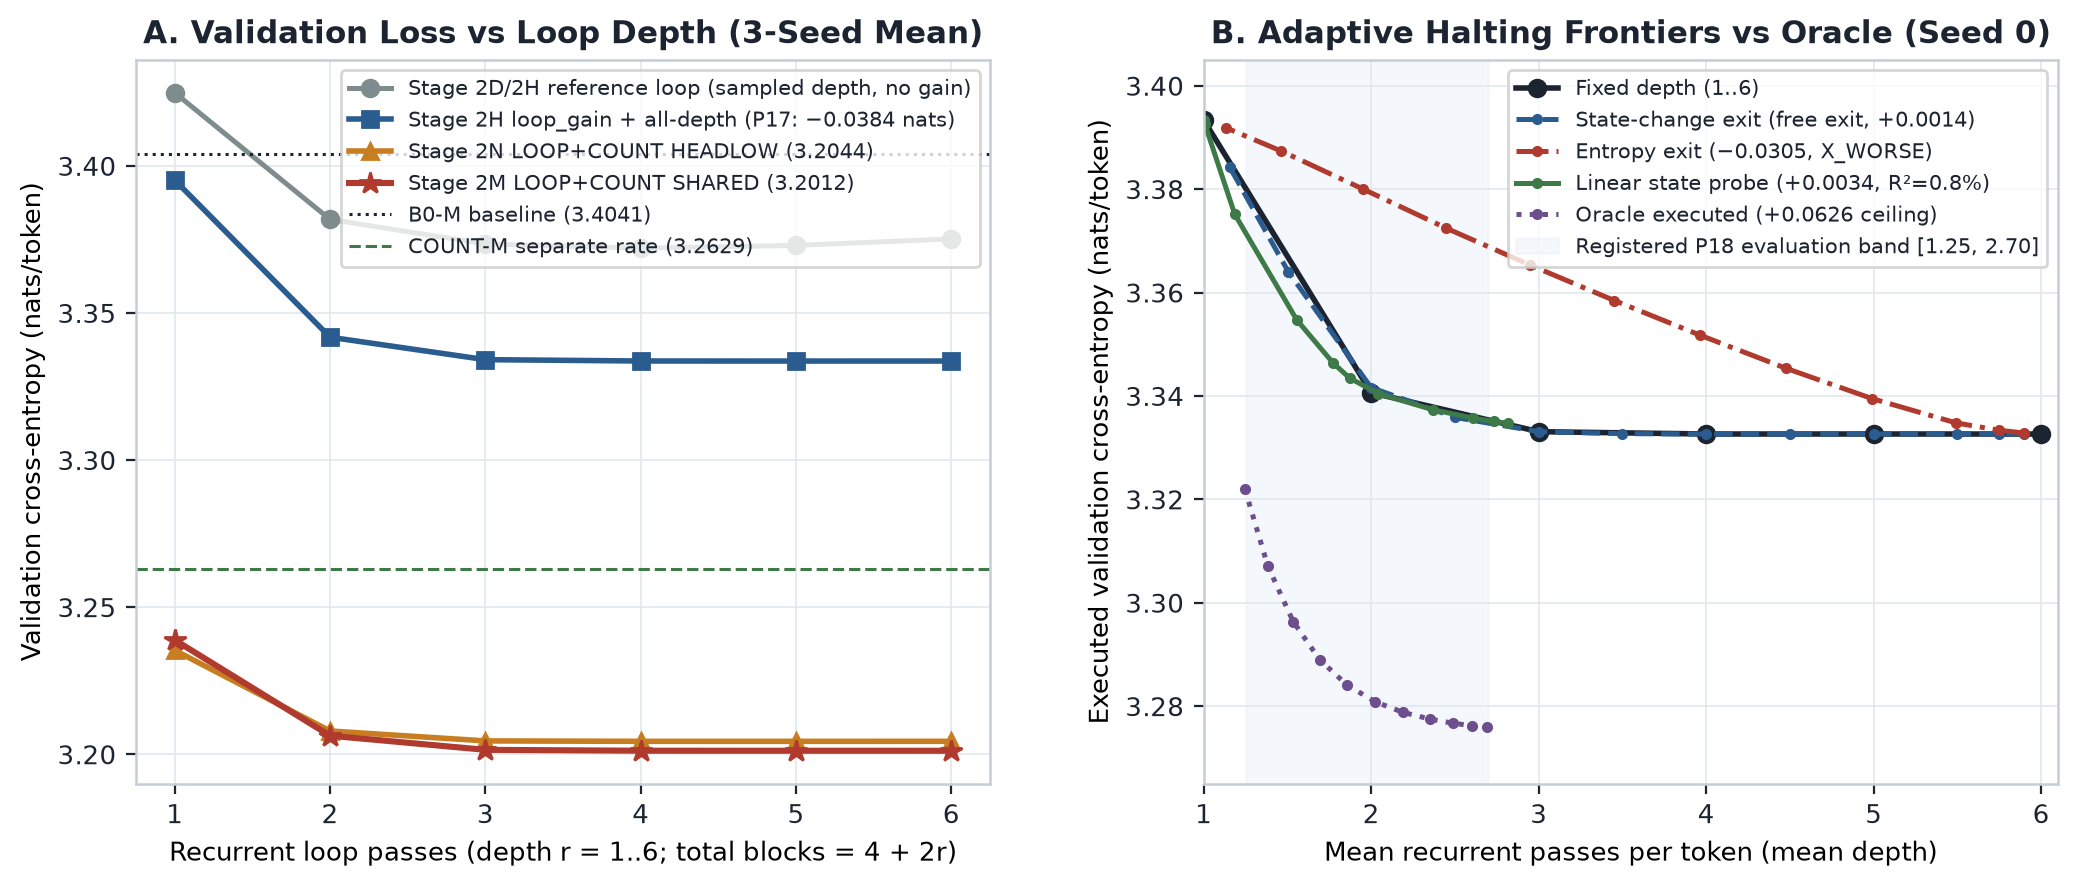
\includegraphics[width=0.98\textwidth]{../docs/figures/fig4_loop_depth_and_halting.png}
    \caption{(A) Validation loss across recurrent loop depths $r=1\dots 6$. (B) Stage 2I adaptive halting frontiers vs fixed depth and the executed oracle ceiling.}
    \label{fig:loop}
\end{figure}

\begin{figure}[htbp]
    \centering
    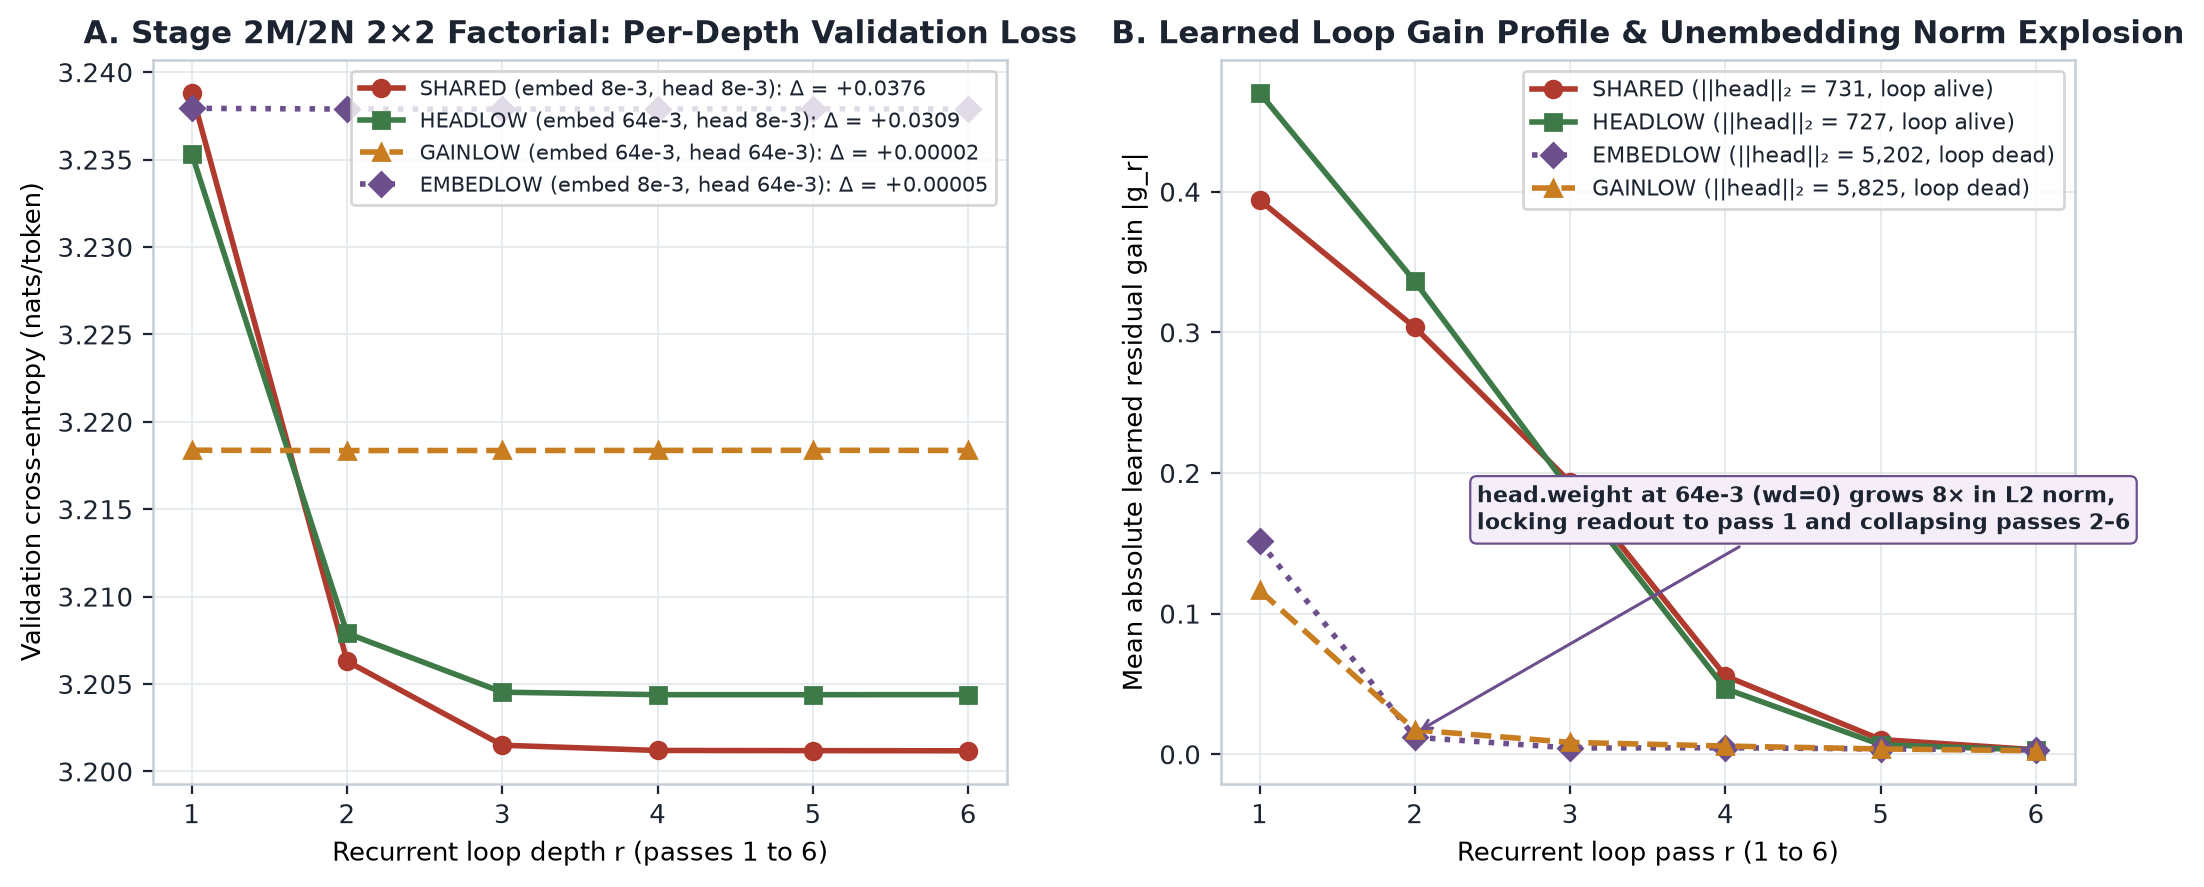
\includegraphics[width=0.98\textwidth]{../docs/figures/fig5_stage2mn_2x2_diagnosis.png}
    \caption{(A) Stage 2M/2N $2\times 2$ factorial per-depth validation loss curves. (B) Learned per-pass $|g_r|$ profiles and \texttt{head.weight} L2 norms showing how \texttt{head.weight} at $64\times 10^{-3}$ explodes $8\times$ and collapses passes 2--6.}
    \label{fig:diag}
\end{figure}

Finally, when Stage 2L combined \texttt{LoopGPT} with \texttt{COUNT} under the separate-rate recipe ($\text{Muon } 8\times 10^{-3}, \text{AdamW } 64\times 10^{-3}$), the COUNT read lowered validation loss by $-0.1722$ nats (P21), but all extra loop passes went completely inert ($\text{depth } 1 = \text{depth } 6$ within $0.00006$ nats). Across Stages 2M and 2N (Figure~\ref{fig:diag}), a $2\times 2$ factorial over $(\text{embeddings LR}) \times (\text{head.weight LR})$ with \texttt{loop\_gain} at $8\times 10^{-3}$ isolated the exact cause:
\begin{itemize}
    \item \textbf{\texttt{GAINLOW} (P22 Refuted, \texttt{embed} $64\times 10^{-3}$, \texttt{head} $64\times 10^{-3}$):} Loop dead (benefit $+0.00002$ nats, $\|\text{head.weight}\|_2 = 5,824.5$).
    \item \textbf{\texttt{EMBEDLOW} (P25 Refuted, \texttt{embed} $8\times 10^{-3}$, \texttt{head} $64\times 10^{-3}$):} Loop dead at seed-0 futility gate (benefit $+0.00005$ nats, $\|\text{head.weight}\|_2 = 5,202.0$).
    \item \textbf{\texttt{HEADLOW} (P24 Supported, \texttt{embed} $64\times 10^{-3}$, \texttt{head} $8\times 10^{-3}$):} Loop alive on all 3 seeds (mean benefit \textbf{$+0.03095$ nats}, best-depth loss \textbf{3.2044}, $\|\text{head.weight}\|_2 = 726.7$, \texttt{X\_BETTER} than \texttt{GAINLOW} by $-0.0140$ nats).
    \item \textbf{\texttt{SHARED} (P23 Supported, \texttt{embed} $8\times 10^{-3}$, \texttt{head} $8\times 10^{-3}$):} Loop alive on all 3 seeds (mean benefit \textbf{$+0.03764$ nats}, best-depth loss \textbf{3.2012}, $3.2015$ at depth 3, $\|\text{head.weight}\|_2 = 731.3$), tying \texttt{HEADLOW} within \texttt{NO\_MEANINGFUL\_DIFFERENCE} ($+0.0032$ nats) and achieving the lowest validation loss in the project (\textbf{$-0.2029$ nats} below \texttt{B0-M}).
\end{itemize}

\begin{table}[htbp]
\centering
\small
\caption{Summary of Key Milestones Across Stages 1 and 2 (200M Tokens, FineWeb-Edu).}
\label{tab:summary}
\begin{tabular}{llrrr}
\toprule
\textbf{Stage / Model Arm} & \textbf{Key Mechanism / Recipe} & \textbf{Backbone Params} & \textbf{Mean Val Loss} & \textbf{Gap vs Baseline} \\
\midrule
Stage 1 \texttt{shuf} & 6-layer GPT + degree-shuffled MB brain & 5.11M (total) & 3.9339 & --- \\
Stage 1 \texttt{real} & 6-layer GPT + FlyWire v783 MB brain & 5.11M (total) & 3.9484 & $+0.0144$ (\texttt{X\_WORSE}) \\
\midrule
Stage 2.0 \texttt{B0-S} & Modern pre-norm GPT, Muon $8\times 10^{-3}$ & 6.82M & 3.5198 & $+0.1158$ vs \texttt{B0-M} \\
Stage 2.0 \texttt{B0-M} & Modern pre-norm GPT, Muon $8\times 10^{-3}$ & 13.76M & 3.4041 & Baseline \\
Stage 2.0 \texttt{B0-L} & Modern pre-norm GPT, Muon $8\times 10^{-3}$ & 29.36M & 3.2610 & $-0.1431$ vs \texttt{B0-M} \\
\midrule
Stage 2G \texttt{B0-M sep} & \texttt{B0-M}, Muon $8\times 10^{-3}$ / AdamW $64\times 10^{-3}$ & 13.76M & 3.3853 & $-0.0188$ vs \texttt{B0-M} \\
Stage 2A \texttt{COUNT-M} & Host-RAM COUNT (LOO), shared $32\times 10^{-3}$ & 13.76M & 3.3242 & $-0.0798$ vs \texttt{B0-M} \\
Stage 2G \texttt{COUNT-M sep} & Host-RAM COUNT (LOO), AdamW $64\times 10^{-3}$ & 13.76M & 3.2629 & $-0.1224$ vs \texttt{B0-M sep} \\
\midrule
Stage 2D/2H \texttt{loop ref} & \texttt{LoopGPT} ($r\le 6$), sampled depth & 13.76M & 3.3720 & $-0.0321$ vs \texttt{B0-M} \\
Stage 2H \texttt{loop both} & \texttt{LoopGPT} + \texttt{loop\_gain} + all-depth loss & 13.76M & 3.3336 & $-0.0705$ vs \texttt{B0-M} \\
Stage 2M \texttt{GAINLOW} & \texttt{LoopGPT+COUNT}, \texttt{head/embed} $64\times 10^{-3}$ & 13.76M & 3.2184 & Loop dead ($+0.00002$) \\
Stage 2N \texttt{HEADLOW} & \texttt{LoopGPT+COUNT}, \texttt{head} $8\times 10^{-3}$, \texttt{embed} $64\times 10^{-3}$ & 13.76M & 3.2044 & Loop alive ($+0.03095$) \\
\textbf{Stage 2M \texttt{SHARED}} & \textbf{\texttt{LoopGPT+COUNT}, all AdamW $8\times 10^{-3}$} & \textbf{13.76M} & \textbf{3.2012} & \textbf{$-0.2029$ vs \texttt{B0-M}} \\
\bottomrule
\end{tabular}
\end{table}

\section{Conclusion}

Across 16 pre-registered stages, literal connectome wiring (\texttt{Stage 1}), in-network similarity hash backoffs (\texttt{Stage 2B}), learned memory gates under tuned unembedding rates (\texttt{Stages 2K--2K2}), and causal per-token halting policies (\texttt{Stage 2I}) all failed to beat simpler controls. Conversely, three hardware-aligned mechanisms delivered large, reproducible gains: (1) \textbf{exact host-RAM $n$-gram memory (\texttt{COUNT}) with online leave-one-out subtraction} ($-0.1224$ nats, matching $2.1\times$ larger backbones at zero VRAM cost), (2) \textbf{one-shot count writes with context-gated overlays (\texttt{GatedOverlay}, $81\%\text{--}95.4\%$ interference reduction) and memory-on KL consistency consolidation} ($0.750$ consolidated recall, zero forgetting), and (3) \textbf{all-depth recurrent looping with learned per-pass residual gains (\texttt{loop\_gain}) and restrained unembedding learning rates} ($-0.2029$ nats combined reduction below \texttt{B0-M}).

\end{document}
